\section{Results}

\subsection{Psychometric results}
 
The SBT experiment, performed in seven subjects, tested the accuracy and precision of SBT percepts, near upright (SBT0), at 45\textdegree and 90\textdegree right side down (SBT45 and SBT90), and at 45\textdegree and 90\textdegree left side down (SBT-45 and SBT-90). The same subjects also performed the SVV experiment, tested at nine roll-tilt angles, ranging from -120 to 120\textdegree in 30\textdegree intervals. Figure 3 shows the results of a typical subject (S1) in both tasks. The top panels show the proportion of CW responses for the five SBT tasks, relative to the reference orientation. For an ideal observer, all psychometric functions would resemble a step centered at zero. Across the five reference orientations (0\textdegree, {\textpm}45\textdegree, or {\textpm}90\textdegree), the psychometric data indicate underestimations and overestimations of perceived body angle, but no consistent bias, which resembles previous reports \cite{mittelstaedt1983, mast1996, jarchow1999, vanbeuzekom2001} that body-tilt perception is accurate on average. We fitted psychometric curves through these data (see Materials and Methods, Eq. 1), to obtain estimates for the mean ($\mu$), SD ($\sigma$), and lapse rate ($\lambda$). Parameter $\mu$ is a measure for the accuracy of the subject's body-tilt percept. Perceptual variability, inversely related to precision, is reflected by $\sigma^2$, whereas the lapse rate ($\lambda = 0.06$) accounts for stimulus-independent errors \cite{wichmann2001}. In all five SBT tasks, the $\mu$ values are relatively close to the veridical reference orientation (0\textdegree, 45\textdegree, or 90\textdegree), i.e., errors are <5\textdegree. The psychometric fits further show that variability is lower in the SBT0 task, with s = ~4\textdegree, than in the SBT±45 and SBT±90 task, where s = ~10\textdegree. 

\begin{figure}
    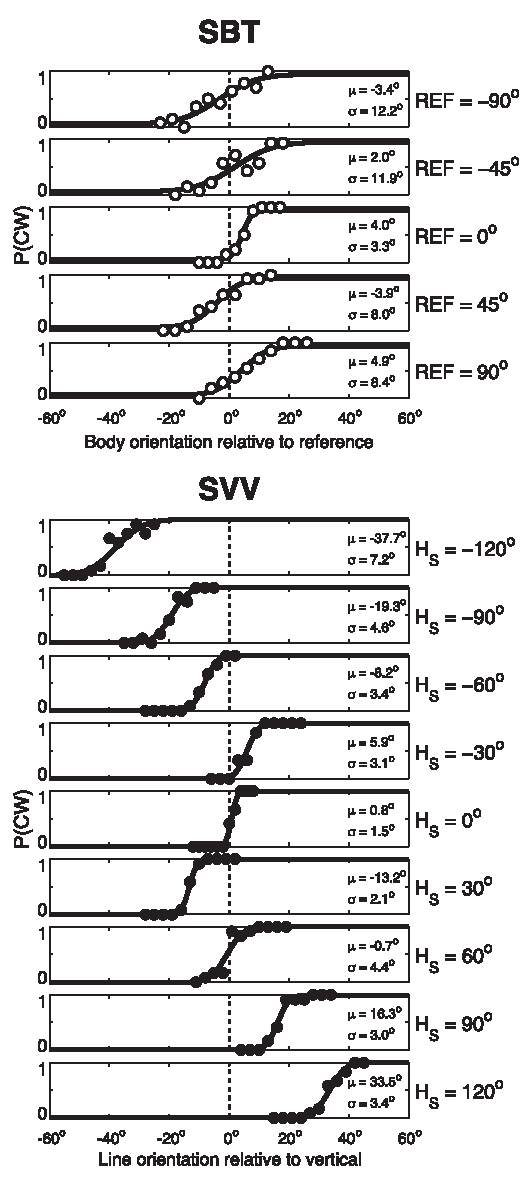
\includegraphics[width=0.5\textwidth]{src/paper1/figure3.pdf}
    
    \caption{SBT versus SVV performance in one subject (S1). Top, SBT. Proportion of CW responses is plotted against body orientation relative to the reference orientation (0\textdegree, \textpm45\textdegree, or \textpm90\textdegree). $\mu > 0\degree$ indicates tilt underestimation. Bottom, SVV. Proportion of CW responses is plotted against line orientation relative to vertical. Solid lines, Best-fit cumulative Gaussians, typified by $\mu$ and $\sigma$.}  
    \label{p1:fig3}
\end{figure}

The bottom section of Figure 3 illustrates the performance of the same subject in the SVV task. Each panel demonstrates how the fraction of CW responses changes as a function of line orientation relative to the perceived vertical, for each tilt angle tested. Performance is very accurate in the upright condition. For moderate body tilts, i.e., 30∞, this subject shows small systematic errors, indicating that the line must be set in a direction opposite to the head tilt to be perceived vertical in space. For larger tilts (=60∞), systematic errors occur with increasing tilt angle, with amplitudes up to 40\textdegree, as if tilt is underestimated. This response pattern is consistent with previous literature \cite{aubert1861, udodehaes1970, mittelstaedt1983, vanbeuzekom2000}. Close scrutiny also reveals that the precision in the vertical percept deteriorates away from the upright position. 

Psychometric fits capture these observations. In the upright position, the percept of visual vertical is virtually unbiased, as indicated by a µ value of 0.8∞. At large tilts, e.g., at -120\textdegree and 120\textdegree, $\mu = -37.7\degree$ and $\mu = 33.5\degree$, respectively, which means that the line must be tilted away from true vertical to be perceived as vertical in space. Furthermore, the fitted psychometric curves are steepest at 0\textdegree tilt, reflected by $\sigma = 1.5\degree$. With larger tilt angles, $\sigma$ increases, reaching maximum values of 7.2\textdegree and 4.3\textdegree at tilts of -120\textdegree and +120\textdegree, respectively. 

The results of this subject are exemplary for all subjects, as shown by the bias and SD data points in Figure 4. The mean results across the seven subjects are shown in the rightmost column. The bold lines in Figure 4 represent the fits from our Bayesian model, which will be discussed later in this section. 

\begin{figure}
	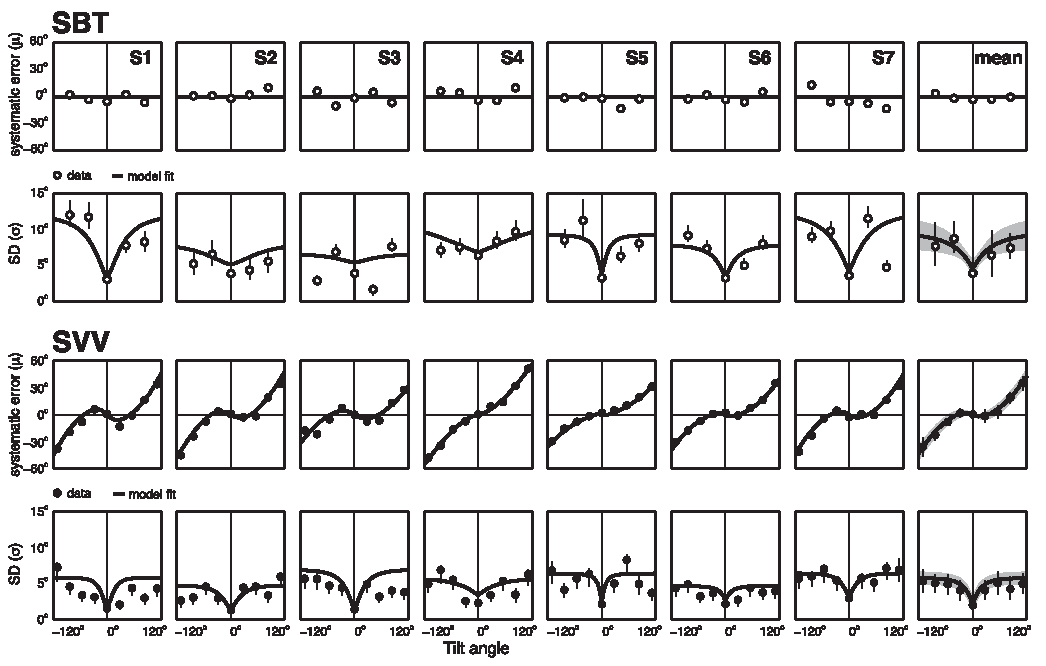
\includegraphics[width=1.0\textwidth]{src/paper1/figure4.pdf}
	
    \caption{Model predictions superimposed on parameters from the psychometric fits to the SBT (two top rows) and SVV data (two bottom rows). Accuracy and variability characteristics as a function of roll-tilt angle are shown; values are psychometric fits ($\mu$ and $\sigma$ values, [CIRCLES]) and model predictions (line) from all subjects. Mean data and mean predictions across subjects are plotted in the rightmost column.}
    \label{p1:fig4}
\end{figure}

The two top rows in Figure 4 show the accuracy ($\mu$) and precision ($\sigma$) of SBT percepts, now plotted against body orientation. For each subject, these values ($\mu$ and $\sigma$) were derived from the fitted cumulative Gaussian curves (Fig. 3). Biases for SBT, shown in the top row of Figure 4, indicate moderate deviations in either direction from perfect performance, but no systematic pattern emerges. Across the seven subjects, the $\mu$ values ranged from -14.2\textdegree to +11.7\textdegree across the five SBT tasks. On average, however, there was no systematic bias for the five body orientations (ANOVA; F(4,24) = 1.4; p = 0.25), as also indicated by the rightmost panels. The data further show that, in all subjects, variability is statistically lower ($p < 0.05$) at the upright orientation, with s values <4∞, than in the tilted conditions (45\textdegree and 90\textdegree), with $\sigma$ values ranging up to ~12∞. 

The two bottom rows of Figure 4 summarize our SVV data across the entire tilt range. Accuracy is close to perfect at upright orientation in all subjects, with mean values ranging between 0.1∞ and 2.8∞. For tilts =60∞, all subjects show systematic SVV errors (biases) of undercompensation, ranging up to maximum values close to 60∞. Three subjects (S1, S2, and S3) also show slight errors of overcompensation in the smallest tilt range (<60∞). The variability in the SVV is <3.0∞ for upright, which is consistently lower than in the tilted conditions, where variability reaches values ranging up to 8∞. 

Together, the results in Figure 4 show that SVV and SBT have different accuracy and precision characteristics. Subjects perceive their body-tilt angle more accurately than the spatial orientation of the visual line. However, when it comes to variability, performance is reversed: SVV curves are narrower than the SBT curves in all subjects, at both tilt angles, meaning that they are consistently less variable in the SVV task than in the SBT task. 

\subsection{Model predictions}

The bold lines in Figure \ref{p1:fig4} present the predictions of the Bayesian integration model, fitted simultaneously to the original responses from the SBT and SVV tasks. The rightmost column of Figure \ref{p1:fig4} shows the mean predictions from this model superimposed on the averaged parameters from the psychometric fits, indicating that the sensory integration model can account very well for all the characteristics of the data. 

By design (see Materials and Methods), the sensory integration model fits a horizontal fit line through µSBT = 0∞ because it cannot account for the small systematic SBT errors. As to SBT precision, the model predictions show an increase of noise with tilt angle similar to the actual increase of noise between 0∞ and 90∞ tilt, for all subjects. These model fits further suggest that the increase of SBT noise is steepest at small tilt angles and levels off at larger tilts. According to the model, the increase of SBT noise with tilt angle is attributable to the corresponding increase of noise in the head sensors (parameter aHS), but levels off by the constant noise level in the body sensors. The third row in Figure 4 depicts the model predictions of the systematic SVV errors, which show a very good match. Also with respect to SVV variability, fits and data show similar trends, suggesting an increase of SVV noise with tilt angle, which levels off at larger tilts. 

For each subject, best-fit parameter values and their bootstrap-based SD levels are listed in Table \ref{p1:tab1}. Parameter bHS, representing the noise (sHS) in the otolith signal in the upright subject, ranges between 1.1∞ and 3.9∞. Best-fit values of parameter aHS are significantly positive (p < 0.05) for all subjects, ranging from 0.07∞/∞ (S4) to 0.23∞/∞ (S1). This implies that the noise in the otoliths increases with tilt angle. The width of the head-in-space prior (sHSP) ranges from 9.4∞ (S2) to 18.7∞ (S5), with a mean of 12.5 ± 3.2∞, consistent with our previous report \cite{devrijer2009}. Best-fit values of parameter sBS, reflecting the noise in the sensory body-in-space signal, range from 6.7∞ (S3) to 15.0∞ (S5), with a mean of 10.8 ± 3.1∞, which is about twice as large as the best-fit values of parameter sHB, reflecting noise in the head-on-body signal, ranging from 1.8∞ (S6) to 9.3∞ (S3), with a mean of 4.9 ± 2.7∞. Thus, the parameter fits imply that the neck sensors are more precise than the body-tilt sensors. As has been discussed extensively in our previous paper \cite{devrijer2009}, the amplitude of uncompensated ocular counterroll (AOCR) shows large intersubject variability. 

\begin{table}

\begin{tabular}{lllllll}
\hline
Subject & $a_{HS}$ (\textdegree/\textdegree) & $b_{HS}$ (\textdegree) & $\sigma_{HSP}$ (\textdegree) & $\sigma_{BS}$ (\textdegree) & $\sigma_{HB}$ (\textdegree) & $A_{OCR}$ (\textdegree) \\
\hline
S1 & 0.23 \textpm 0.02 & 1.2 \textpm 0.32 & 11.6 \textpm 1.0 & 12.3 \textpm 1.1 & 3.3 \textpm 1.2 & 27.0 \textpm 2.2 \\
S2 & 0.12 \textpm 0.02 & 1.2 \textpm 0.52 & 9.4 \textpm 1.1 & 8.4 \textpm 2.9 & 6.4 \textpm 4.1 & 17.0 \textpm 3.8 \\
S3 & 0.20 \textpm 0.03 & 1.1 \textpm 0.42 & 14.4 \textpm 1.7 & 6.7 \textpm 1.9 & 9.3 \textpm 2.4 & 17.5 \textpm 2.1 \\
S4 & 0.07 \textpm 0.50 & 3.9 \textpm n/a & 11.2 \textpm 1.3 & 12.6 \textpm 2.3 & 7.1 \textpm 3.5 & 0 \textpm n/a \\
S5 & 0.11 \textpm n/a & 3.3 \textpm 1.0 & 18.7 \textpm 4.8 & 15.0 \textpm n/a & 3.6 \textpm 2.1 & 1.06 \textpm n/a \\
S6 & 0.23 \textpm 0.09 & 3.0 \textpm 1.5 & 9.5 \textpm 1.1 & 8.0 \textpm 0.83 & 1.8 \textpm n/a & 18.8 \textpm 4.1 \\
S7 & 0.20 \textpm 0.14 & 3.2 \textpm 1.0 & 12.8 \textpm 2.4 & 12.7 \textpm 6.1 & 3.0 \textpm n/a & 20.8 \textpm 9.0 \\
Mean & 0.16 \textpm 0.06 & 2.4 \textpm 1.2 & 12.5 \textpm 3.2 & 10.8 \textpm 3.1 & 4.9 \textpm 2.7 & 14.6 \textpm 10.2 \\
\hline
\multicolumn{7}{l}{Imposed fit limits were as follows: $a_{HS}$: 0.5\textdegree/\textdegree; $b_{HS}$, $\sigma_{HSP}$, $\sigma_{BS}$, $\sigma_{HB}$, 50\textdegree; $A_{OCR}$, 30\textdegree. SD values are not shown (n/a) when bootstrapped values formed a skewed distribution. $a_{HS}$, Tilt-related increase in otolith noise; $b_{HS}$, otolith noise in upright position; $\sigma{HSP}$, width of head-tilt prior; $\sigma{BS}$, noise in body-in-space sensors; $\sigma{HB}$, noise in neck sensors; $A_{OCR}$, uncompensated ocular counterroll.} \\
\end{tabular}

\caption{Best-fit parameter and bootstrap-based SD values}
\label{p1:tab1}
\end{table}

\subsection{Sensory weights}
 
To obtain the model fits in Figure \ref{p1:fig4}, we made the assumption (see Introduction) that information from both direct and indirect pathways (Fig. \ref{p1:fig1}) is used to estimate body and head orientation in space. The sensory weights, indicating the relative contribution of both pathways, can be computed from the fit results in Table 1. To obtain the body-in-space estimate, necessary for the SBT, the model uses both direct information from the body sensors and indirect information from the combination of otolith and neck information. Because the variability of the otolith signal (sHS) increases with tilt angle (aHS > 0), as shown in Table 1, the relative importance of direct and indirect pathways becomes dependent on tilt angle. This can be seen in Figure 5(top row), which shows the relative weights of these signals for each subject, derived from Equation 2 and the best-fit parameter values in Table 1. The mean (±SD) pattern across subjects is shown in the rightmost pattern. 

\begin{figure}
    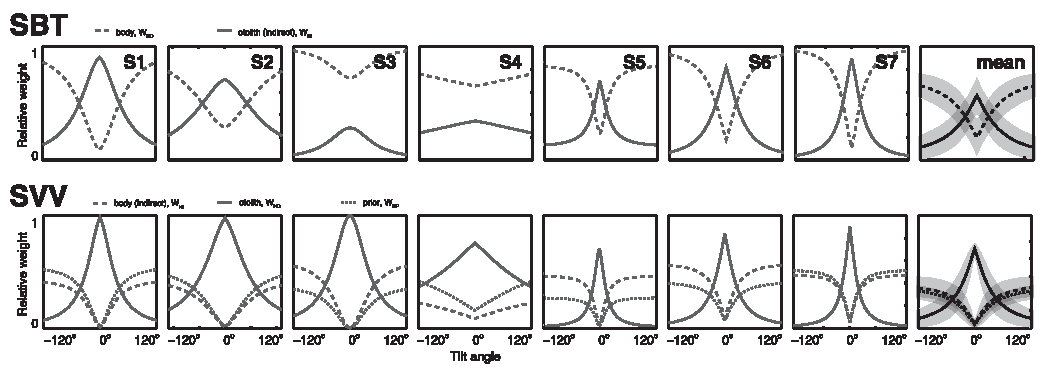
\includegraphics[width=1.0\textwidth]{src/paper1/figure5.pdf}
    
    \caption{Tilt dependence of weight factors in SBT (top) and SVV (bottom) for each subject. Trends with tilt angle are similar for all subjects. Head-in-space prior is only involved in SVV computations. Means across subjects are plotted in the rightmost column.}
\end{figure}

Instead of an overall dominance of body receptors in the direct pathway, the model implies that it is actually the indirect pathway, carrying the otolith signal, that dominates the behaviorally important range near upright. In most of our subjects (S1, S3, S5, S6, and S7), it was only when the otoliths became less reliable, at larger tilts, that the body sensors (direct pathway) got the upper hand (wBD > 0.5). 

For the SVV task, the model assumes that both information from the otoliths (direct) and the combination of body and neck information (indirect) is used. Figure 5 (bottom row) illustrates the relative contributions from these sensors as well as from the prior, based on the model fits (Table 1) and Equation 6. The SVV pattern looks similar to the SBT pattern (Fig. 5, top row): in all subjects, the otoliths are very dominant near upright, with weights close to 1, but their contribution declines when tilt angle increases. As we saw for the SBT signal weights, this decline reflects increasing otolith noise levels. In the SVV, the decline is steeper than in the SBT, where the reference frame transformation leads to an enhanced noise level with a less pronounced tilt dependence. As the otolith contribution decays, the contributions of the prior and indirect pathway become more manifest. According to our model fits, the weight of the body sensors in the SVV task (wHI) at 90∞ tilt ranges between 0.19 (S4) and 0.53 (S6). 

\subsection{Model evaluation}
 
To test whether the assumption of indirect pathways in the model is warranted, we compared its performance with a reduced version with only direct pathways (see Materials and Methods). With this in mind, we performed a likelihood ratio test of the complete model fit (with direct and indirect pathways) versus the fit of a model with direct pathways only [i.e., SVV just based on head sensors (the otoliths), the SBT just based on body sensors]. The results are shown in Table 2. For each subject, the complete model provided a significantly better account of the data than the reduced model without multisensory integration through the indirect pathways. In other words, head, neck and body sensors all contribute to both SBT and SVV. 

\begin{table}
\begin{tabular}{llllll}
\hline
Subject & MLE full model & MLE reduced model & $p$ & BIC full model & BIC psychometric fits \\
\hline
S1 & 231.5 & 312.4 & \textless 0.001 & 498.1 & 540.3 \\
S2 & 197.8 & 216.9 & \textless 0.001 & 430.6 & 539.3 \\
S3 & 267.5 & 313.4 & \textless 0.001 & 570.0 & 548.2 \\
S4 & 207.5 & 218.2 & \textless 0.001 & 450.0 & 569.1 \\
S5 & 195.6 & 216.3 & \textless 0.001 & 426.2 & 571.0 \\
S6 & 163.5 & 183.2 & \textless 0.001 & 362.0 & 502.5 \\
S7 & 248.0 & 260.0 & \textless 0.001 & 531.1 & 633.5 \\ 
\hline
\multicolumn{6}{l}{Log-likelihood ratio test of the full model (with indirect pathways) and reduced model (without indirect pathways). For all subjects, the full model outperforms the reduced model lacking multisensory integration through the indirect pathways. BIC values are much lower for the Bayesian integration model compared with separate psychometric fits in six of seven subjects.} \\
\end{tabular}
\caption{Validation of the model}
\label{p1:tab2}
\end{table}


We also compared our model, which provides a mechanistic explanation of the full dataset, with the pure descriptive account of the data as obtained by fitting separate psychometric curves to the data for the five SBT angles and nine SVV angles (Eq. \ref{p1:eqn1}, Fig. \ref{p1:fig3}, and \nameref{p1:sec:methods}, Model evaluation). Maximum-likelihood estimates were calculated and corrected for the number of free parameters using the BIC. As shown in Table 2, we found the lowest BIC values, indicating a better model, for the Bayesian model in all subjects, except S3. One might argue that the mean corrections before fitting the Bayesian model added another nine parameters that should be taken into account when comparing the models, even though these parameters were not fitted by the model. However, even for the worst-case scenario of 16 parameters, our Bayesian model still outperformed the individual psychometric fits (BICmechanistic = 3583 < BICpsychometric = 3910). 

\subsection{Model validation}
 
To further validate the model, we independently tested one of its predictions that can be assessed experimentally in isolation: head-on-body variance. In supine position, subjects judged their head orientation (CW/CCW) relative to the body midline after it had been passively roll-rotated with speeds subthreshold for the canals to various angles (see \nameref{sec:methods}, Model validation: independent test of neck noise). Psychometric fits indicate no systematic bias in these head-on-body percepts (data not shown). Figure 6 depicts the experimental noise levels derived from these psychometric fits and the predicted values provided by the model, including their 95\% confidence intervals. Because the variance of the estimates increases with the average head-on-body percept, we performed a regression on the log-transformed data \cite{hopkins2000}. The significant correlation between predicted and measured neck noise levels (slope, 1.03; intercept, -0.1; p = 0.04) provides an independent confirmation of the proposed model. 

%\begin{figure}
\begin{wrapfigure}{l}[5pt]{0.5\textwidth}
    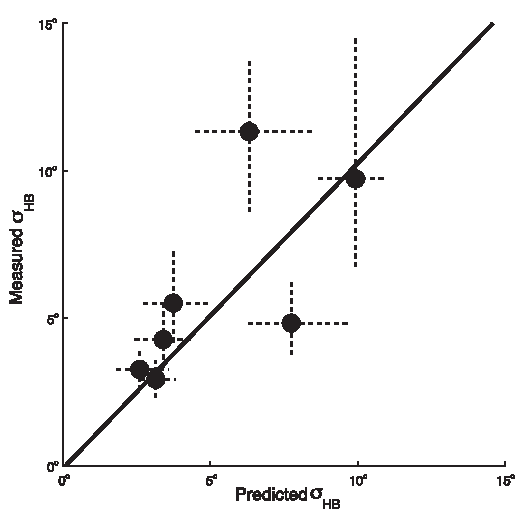
\includegraphics[width=0.5\textwidth]{src/paper1/figure6.pdf}
%\end{figure}
\end{wrapfigure}